%% ============================================================
%% SUBMISSION NOTE:
%% Compiles as-is with pdflatex (standard texlive).
%% For IEEE submission, replace lines 12--26 with:
%%   \documentclass[conference]{IEEEtran}
%%   \IEEEoverridecommandlockouts
%% and remove the FALLBACK PREAMBLE block.
%% Replace the \twocolumn[{...}] title block with \maketitle,
%% and use \begin{abstract} / \begin{IEEEkeywords} environments.
%% Install IEEEtran: sudo apt install texlive-publishers
%% ============================================================

%% --- FALLBACK PREAMBLE (remove when using IEEEtran) ---
\documentclass[10pt,twocolumn,a4paper]{article}
\usepackage[a4paper,top=19mm,bottom=43mm,
            left=14.3mm,right=14.3mm,columnsep=4.2mm]{geometry}
\usepackage{times}
\usepackage{titlesec}
\titleformat{\section}
  {\normalfont\normalsize\bfseries\scshape\centering}{\Roman{section}.}{0.5em}{}
\titlespacing{\section}{0pt}{8pt}{4pt}
\titleformat{\subsection}
  {\normalfont\normalsize\itshape}{\Alph{subsection}.}{0.5em}{}
\titlespacing{\subsection}{0pt}{6pt}{2pt}
\setlength{\parindent}{3.5mm}
\setlength{\parskip}{0pt}
%% --- END FALLBACK PREAMBLE ---
\raggedbottom

% ---- Packages ----
\usepackage{amsmath}
\usepackage{amssymb}
\usepackage{mathtools}
\usepackage{graphicx}
\usepackage{float}
\usepackage{hyperref}
\usepackage{booktabs}
\usepackage{array}
\usepackage{cite}

\hypersetup{colorlinks=true,linkcolor=black,citecolor=black,urlcolor=black}

% ---- Title ----
\title{\vspace{-1em}\textbf{Exam-Induced Cognitive Collapse as a
Working Memory Hijacking: A Psychologically Grounded
Dynamical Systems Model}}
\author{Parth Mehta\\[2pt]
  \small\textit{BITS Pilani, India}}
\date{}

% ================================================================
\begin{document}

\twocolumn[{%
  \maketitle\vspace{-1em}
  \begin{center}\begin{minipage}{0.95\linewidth}
    \small
    \noindent\textbf{\textit{Abstract---}}\textit{%
    This paper presents a dynamical systems model of the
    ``exam-time blackout,'' the sudden collapse of recall efficiency
    under examination conditions. The model is built entirely from
    established psychological constructs: physiological stress $S(t)$,
    recall efficiency $R(t)$, and rumination load $L(t)$ - the fraction
    of working memory occupied by anxiety-driven intrusive thoughts.
    Working memory capacity is treated as a quasi-static function,
    $W(S)=1/(1+k_w S)$ following Baddeley's model. The $R$-$L$
    subsystem forms a mutual inhibition loop grounded in Eysenck's
    Attentional Control Theory and Anderson's retrieval-induced
    forgetting: successful recall suppresses rumination, and rumination
    crowds recall out of working memory. This toggle-switch topology
    produces cascade collapse dynamics not achievable with simpler
    coupling structures. Numerical simulation demonstrates that the
    model correctly reproduces the Yerkes-Dodson inverted-U
    relationship between arousal and performance, the cascade collapse
    triggered by a single difficult question, graded sensitivity to
    prior exam experience, and spontaneous post-exam recovery.
    An analytical first-order bound on blackout severity,
    $R_{\min} \approx R_F(1 - A\,\Delta S)$ where
    $A = \delta\sigma/(\beta+\nu)$, is derived and verified
    numerically. Three control-theoretic interventions are derived
    directly from the model's parameter structure.}

    \medskip\noindent\textbf{\textit{Keywords---}}%
    Dynamical Systems, Working Memory, Attentional Control Theory,
    Yerkes-Dodson Law, Rumination, Cognitive Collapse.
  \end{minipage}\end{center}\bigskip
}]

% ================================================================
\section{Introduction}

The sudden failure of memory retrieval under examination conditions
is a phenomenon reported universally by students. One moment the
mind is an ordered repository of studied material, the next it is
entirely blank. Informally termed the ``exam blackout,'' this
experience is typically attributed to anxiety or insufficient
preparation. These explanations are descriptive rather than
mechanistic. They fail to account for the characteristic suddenness
of the collapse, its dependence on specific events within the
exam, a single hard question can trigger the persistence of
the blank state despite intact long-term memory, and the equally
sudden recovery that follows the exam's conclusion.

Dynamical systems theory offers a natural vocabulary for modelling
such state transitions. The challenge is ensuring that the variables
and coupling terms chosen correspond to real psychological mechanisms
rather than convenient mathematical abstractions. Long-term memory
does not become globally inaccessible as a smooth continuous
variable. What changes under stress is working memory
\emph{capacity} and \emph{allocation}, two constructs with
extensive empirical grounding~\cite{baddeley1986,eysenck2007}.
When the model is built from these constructs, the dynamics naturally 
produce the empirical phenomena that the blackout experience exhibits.

This paper develops such a model. The three state variables are
physiological stress $S(t)$, recall efficiency $R(t)$, and
rumination load $L(t)$. The coupling between $R$ and $L$ is a
mutual inhibition loop: recall suppresses rumination via a
retrieval-induced forgetting~\cite{anderson2003}, and rumination
suppresses recall by occupying working memory~\cite{eysenck2007}.
This toggle-switch topology is the structural basis for cascade
dynamics. A stress perturbation that temporarily reduces $R$
weakens the $-\tau RL$ suppression of $L$; $L$ then rises,
further suppressing $R$ through the working memory bottleneck,
creating a self-reinforcing collapse.

The remainder of this paper is structured as follows.
Section~\ref{sec:bg} reviews the psychological literature grounding
each modelling choice. Section~\ref{sec:model} presents the
governing equations. Section~\ref{sec:analysis} analyses the fixed
points, cascade mechanism, and analytical severity bound.
Section~\ref{sec:results} presents numerical simulation results.
Section~\ref{sec:control} discusses control-theoretic interventions.
Section~\ref{sec:conclusion} concludes.

% ================================================================
\section{Background and Related Work}
\label{sec:bg}

\subsection{Yerkes-Dodson Law}

The inverted-U relationship between arousal and performance,
established by Yerkes and Dodson~\cite{yerkes1908}, is the most
replicated finding in the stress-performance literature. Performance
improves from low to moderate arousal (heightened alertness and
focus) and deteriorates from moderate to high arousal (overwhelm
and cognitive narrowing). Any mechanistic model of exam performance
would reproduce this shape: at zero stress there is insufficient
drive to focus, at very high stress there is insufficient working
memory capacity for retrieval.

\subsection{Working Memory Capacity}

Baddeley's working memory model~\cite{baddeley1986} establishes
that the cognitive workspace available for active processing is
strictly limited in capacity and degrades under high arousal. This
is not a property of long-term memory storage but of the retrieval
and manipulation system. Working memory capacity is modelled here
as the quasi-static function $W(S) = 1/(1+k_w S)$: full capacity
at zero stress, monotonically decreasing with arousal. This
coupling, dividing the maximum recall rate $\rho$ by the working
memory denominator directly produces the Yerkes-Dodson inverted-U
in recall: moderate stress provides alertness while leaving
sufficient capacity, high stress collapses capacity faster than
the alertness benefit accumulates.

\subsection{Attentional Control Theory}

Eysenck's Attentional Control Theory~\cite{eysenck2007} provides
the leading mechanistic account of how anxiety impairs cognitive
performance. The central claim is that anxiety generates
task-irrelevant intrusive thoughts like worry about failure,
self-evaluation, social comparison that competes with
task-relevant processing for the finite capacity of working memory.
Performance degrades not because knowledge is lost from long-term
memory but because the cognitive workspace is occupied by
anxiety-driven rumination, leaving insufficient capacity for
retrieval. This motivates the rumination variable $L(t)$: a
continuous measure of the fraction of working memory occupied by
intrusive thoughts. The coupling term $\sigma S(1-L)$ in the
rumination equation directly encodes Eysenck's mechanism: stress
generates intrusive thoughts at a rate proportional to current
arousal, with logistic saturation at $L=1$.

\subsection{Retrieval-Induced Forgetting}

Anderson and Levy~\cite{anderson2003} demonstrated that successful
retrieval actively suppresses competing memory representations,
including emotional and anxious content. In the exam context,
successfully recalling an answer suppresses the intrusive thoughts
competing for the same working memory space. This establishes the
negative coupling from $R$ to $L$: the term $-\tau RL$ in the
rumination equation encodes active recall driving rumination
out of working memory. This coupling, combined with the $(1-L)$
factor suppressing recall in the recall equation, creates the
mutual inhibition loop that is the structural core of the model.

\subsection{Self-Efficacy and Prior Performance}

Bandura's self-efficacy theory~\cite{bandura1977} establishes that
belief in one's own ability, shaped by prior performance
history directly modulates the physiological stress response to
performance situations. A student with a history of exam failure
enters an examination with an elevated baseline arousal, reducing
the perturbation required to trigger a blackout cascade. This is
captured by the prior performance index $E\in[-1,1]$ in the stress
equation: negative values (poor history) raise effective baseline
stress, positive values (good history) lower it.

\subsection{Catastrophe Theory and Cognitive Load}

Thom's catastrophe theory~\cite{thom1975}, extended to performance
modelling by Zeeman~\cite{zeeman1976}, provides the mathematical
precedent for modelling sudden performance collapse as a
bifurcation in a system with control parameters. The present model
is consistent with this framework: the stress perturbation
$\Delta S$ plays the role of the splitting factor, and the cascade
sensitivity $A$ governs the steepness of the system's response.
Cognitive Load Theory~\cite{sweller1988} identifies working memory
capacity limits as the source of performance failure under high
cognitive load. The present model extends this by treating capacity
as the dynamic function $W(S)$ coupled to the stress state, and
by specifying the mechanism - rumination occupancy, through which
that capacity is consumed during an examination.

% ================================================================
\section{State Space and Governing Equations}
\label{sec:model}

\subsection{State Variables}

The model uses three dynamical state variables and one quasi-static
derived quantity, analysed within the phase-space framework of
nonlinear dynamics~\cite{strogatz2018}:
\begin{itemize}
  \item $S(t) \geq 0$: physiological stress / arousal level,
  \item $R(t) \in [0,1]$: recall efficiency (cue\allowbreak-\allowbreak target retrieval strength),
  \item $L(t) \in [0,1]$: rumination load (fraction of working
    memory occupied by intrusive thoughts),
  \item $W(S) = 1/(1+k_w S)$: working memory capacity, quasi-static
    in $S$~\cite{baddeley1986}.
\end{itemize}
Long-term memory storage is held constant throughout. The model
describes how retrieval access is mediated by finite working
memory, which collapses and recovers under exam-induced time pressure.

\subsection{Time Pressure Profile \texorpdfstring{$T(t)$}{T(t)}}

The external driving force is the time pressure profile:
\begin{equation}
  T(t) =
  \begin{cases}
    t/t_{\mathrm{end}}, & t < t_{\mathrm{end}} \\[4pt]
    0,                  & t \geq t_{\mathrm{end}}
  \end{cases}
  \label{eq:T}
\end{equation}
$T(t)$ rises linearly from $0$ to $1$ during the exam, representing
monotonically increasing urgency. The discontinuity at
$t_{\mathrm{end}}$ represents the exam's end and is the mechanism
of post-exam recovery.

\subsection{Governing Differential Equations}

\medskip\noindent\textbf{(1) Stress Dynamics:}
\begin{equation}
  \dot{S} = \alpha T(t) - \beta S - \gamma R - \mu E
  \label{eq:S}
\end{equation}
\begin{itemize}
  \item $\alpha T(t)$: time-pressure amplification, $\alpha>0$
    encodes individual susceptibility to deadline stress,
  \item $-\beta S$: natural physiological stress decay,
  \item $-\gamma R$: successful recall reduces anxiety (confidence
    feedback),
  \item $-\mu E,\;E\in[-1,1]$: prior performance
    bias~\cite{bandura1977}; $E<0$ elevates, $E>0$ reduces
    baseline stress.
\end{itemize}

\medskip\noindent\textbf{(2) Recall Dynamics:}
\begin{equation}
  \dot{R} = \frac{\rho}{1+k_w S}\,(1-L)\,(1-R) - \delta R
  \label{eq:R}
\end{equation}
\begin{itemize}
  \item $\rho W(S) = \rho/(1+k_w S)$: maximum recall rate, gated
    by working memory capacity, produces the Yerkes-Dodson
    inverted-U~\cite{yerkes1908,baddeley1986},
  \item $(1-L)$: rumination occupies working memory, leaving
    fraction $(1-L)$ available for retrieval~\cite{eysenck2007},
  \item $(1-R)$: logistic saturation preventing $R$ exceeding 1,
  \item $-\delta R$: recall fatigue under sustained effort.
\end{itemize}

\medskip\noindent\textbf{(3) Rumination Dynamics:}
\begin{equation}
  \dot{L} = \sigma S(1-L) - \tau R L - \nu L
  \label{eq:L}
\end{equation}
\begin{itemize}
  \item $\sigma S(1-L)$: stress generates intrusive thoughts,
    with logistic saturation at $L=1$~\cite{eysenck2007},
  \item $-\tau R L$: active recall suppresses rumination via
    retrieval-induced forgetting~\cite{anderson2003},
  \item $-\nu L$: passive rumination decay when not under active stress~\cite{borkovec1994}.
\end{itemize}

\subsection{The R--L Mutual Inhibition Loop}

The structural core of the model is the toggle switch between $R$
and $L$. High $R$ drives $\dot{L}$ negative through $-\tau RL$.
High $L$ drives $\dot{R}$ negative through the $(1-L)$ factor.
This mutual inhibition means the system has two competing states:
\emph{functional} (high $R$, low $L$: recall dominates,
rumination suppressed) and \emph{blackout} (low $R$, high $L$:
rumination dominates, recall suppressed). Which state dominates
depends on the balance of timescales and on the amplitude of
stress perturbations the system encounters.

\subsection{Parameter Definitions and Simulation Methodology}

Table~\ref{tab:params} lists all parameters with simulation values.
All simulations used \mbox{\texttt{scipy.integrate.solve\_ivp}} with
the RK45 integrator (\texttt{max\_step}$=0.005$, rtol$=10^{-6}$),
time span $t\in[0,\,5.5]$ with $t_{\mathrm{end}}=3.0$. Initial
conditions are stated with each simulation result.

\begin{table}[h]
\caption{Model Parameters, Psychological Grounding, and Simulation Values}
\label{tab:params}
\centering
\renewcommand{\arraystretch}{1.2}
\begin{tabular}{clc}
\toprule
\textbf{Param.} & \textbf{Description (source)} & \textbf{Value} \\
\midrule
$\alpha$ & Time-pressure sensitivity                        & 0.8  \\
$\beta$  & Stress decay rate                                & 0.4  \\
$\gamma$ & Recall $\to$ stress relief                       & 0.6  \\
$\mu$    & Prior performance weight                         & 0.2  \\
$E$      & Prior performance index, $E\in[-1,1]$            & 0.0  \\
$\rho$   & Max recall rate~\cite{baddeley1986}              & 1.8  \\
$k_w$    & WM stress sensitivity~\cite{baddeley1986}        & 1.0  \\
$\delta$ & Recall fatigue rate                              & 0.25 \\
$\sigma$ & Stress $\to$ rumination rate~\cite{eysenck2007} & 1.2  \\
$\tau$   & Recall $\to$ rumination suppression~\cite{anderson2003} & 1.8  \\
$\nu$    & Passive rumination decay~\cite{borkovec1994}     & 0.35 \\
\bottomrule
\end{tabular}
\end{table}

The parameter values in Table~\ref{tab:params} were chosen to satisfy
three qualitative constraints derived from the psychological literature.
First, the rumination generation rate $\sigma$ must exceed the passive
decay rate $\nu$ ($\sigma=1.2 > \nu=0.35$), ensuring that sustained
stress drives $L$ upward rather than decaying spontaneously as consistent
with Eysenck's observation that exam anxiety is self-sustaining under
pressure~\cite{eysenck2007}. Second, the recall-to-rumination
suppression rate $\tau$ must exceed $\sigma$ ($\tau=1.8 > \sigma=1.2$),
so that successful recall can actively outcompete stress-driven
intrusive thoughts, a necessary condition for the functional state to
be stable, consistent with Anderson's retrieval-induced
forgetting~\cite{anderson2003}. Third, the cascade sensitivity
$A=\delta\sigma/(\beta+\nu)=0.40$ was set to produce a characteristic
perturbation scale $\Delta S^*=1/A=2.5$, placing full blackout at
approximately three times the ambient exam stress level, a moderate
threshold consistent with the clinical observation that most students
do not black out on routine questions but do so under severe
difficulty~\cite{eysenck2007}. The values of $\alpha$, $\gamma$, and
$\mu$ govern the stress equation alone and were set so that the
functional fixed point falls in the physiologically plausible range
$S_F\in[0,\,1]$ for $T\in[0,\,1]$. The model behaviour is robust to
moderate variation in all parameters, the qualitative dynamics
(Yerkes-Dodson compliance, cascade, recovery) are preserved provided
the three ordering constraints above are satisfied.

% ================================================================
\section{Model Analysis}
\label{sec:analysis}

\subsection{Jacobian and Fixed Points}

The Jacobian of the system at any state $(S,R,L)$ is:
\begin{equation}
  J =
  \begin{pmatrix}
    {-\beta} & {-\gamma} & 0 \\[4pt]
    {\scriptstyle\partial_S\dot{R}} &
    {-\rho W(1-L) - \delta} &
    {-\rho W(1-R)} \\[6pt]
    {\sigma(1-L)} & {-\tau L} & {-\sigma S - \tau R - \nu}
  \end{pmatrix}
  \label{eq:jacobian}
\end{equation}
where $\partial_S\dot{R} =
-k_w\rho(1-L)(1-R)/(1+k_wS)^2$.

Numerical root-finding at $T=0.65$ confirms the existence of a
functional fixed point (low $S$, high $R$, low $L$). The Jacobian
eigenvalues at this point are given in Table~\ref{tab:eigenvalues}:
all real parts are negative, confirming local asymptotic stability.

\begin{table}[h]
\caption{Eigenvalues at Functional Fixed Point ($T=0.65$)}
\label{tab:eigenvalues}
\centering
\renewcommand{\arraystretch}{1.25}
\begin{tabular}{lll}
\toprule
\textbf{State} & \textbf{Type} & \textbf{Eigenvalues} \\
\midrule
Functional & Stable spiral & $-0.268,\;\; -2.121 \pm 0.271i$ \\
\bottomrule
\end{tabular}
\end{table}

\subsection{Cascade Mechanism}

The blackout is not caused by instability of the functional fixed
point but is a \emph{trajectory-level cascade}: a stress
perturbation large enough to temporarily weaken the $-\tau RL$
suppression of $L$ initiates a positive feedback loop. As $L$
rises, the $(1-L)$ factor in Eq.~(\ref{eq:R}) reduces $\dot{R}$;
as $R$ falls, the $-\tau RL$ term weakens further, allowing $L$
to grow without restraint. The loop is self-reinforcing until
$R\approx 0$ and $L\approx 1$.

The Jacobian entries $J_{23}=-\rho W(S)(1-R)<0$ and
$J_{32}=-\tau L<0$ form the mutual inhibition pair. Their product
$J_{23}\cdot J_{32}=\tau L\rho W(S)(1-R)>0$ satisfies the
Routh-Hurwitz stability criterion at the functional fixed point.
When this product becomes small, when $L\approx 0$ early in
an exam, or when a shock reduces $R$ toward zero, the restoring
force of the toggle weakens and the system becomes susceptible to
cascade. This explains the clinical observation that a very
difficult question encountered late in an exam, when ambient
stress $S$ is already elevated, is more likely to trigger a
blackout than the same question encountered early.

\subsection{Cascade Threshold: Analytical Bound on Blackout Severity}

After settling to the quasi-static functional fixed point
$(S_F, R_F, L_F)$, a transient stress perturbation of amplitude
$\Delta S$ modelling a difficult question, temporarily raises
$S$ to $S_F+\Delta S$. We derive a first-order bound on the
resulting minimum recall $R_{\min}$.

\medskip\noindent\textbf{Derivation.}
After the shock, $S$ decays at rate $\beta$:
$S(t)\approx S_F + \Delta S\,e^{-\beta t}$.
The excess stress drives additional rumination growth at rate
$\sigma\Delta S(1-L_F)$. Integrating over the decay timescale
with passive loss $\nu$, the peak rumination deviation is:
\begin{equation}
  \Delta L_{\mathrm{peak}} \approx
  \frac{\sigma(1-L_F)\,\Delta S}{\beta + \nu}
  \label{eq:DL}
\end{equation}
Using the functional fixed-point relation
$\delta R_F = \rho W_F(1-L_F)(1-R_F)$, the induced recall drop is:
\begin{equation}
  \Delta R \approx \rho W_F(1-R_F)\,\Delta L_{\mathrm{peak}}
  = \frac{\delta\sigma\,R_F\,\Delta S}{\beta+\nu}
  \label{eq:DR}
\end{equation}
This gives the \emph{cascade threshold formula}:
\begin{equation}
  \boxed{R_{\min}(\Delta S) \approx R_F\!\left(1 - A\,\Delta S\right),
  \qquad A \equiv \frac{\delta\sigma}{\beta + \nu}}
  \label{eq:Rmin}
\end{equation}
The coefficient $A$ is the \emph{cascade sensitivity}: the fraction
of pre-perturbation recall lost per unit stress perturbation. With
the parameters of Table~\ref{tab:params}:
$A = (0.25)(1.2)/(0.4+0.35) = 0.40$.

\medskip\noindent\textbf{Consequences.}
Three implications follow from Eq.~(\ref{eq:Rmin}).

First, \emph{blackout severity scales linearly with perturbation
size} to first order: a harder question causes a proportionally
deeper recall collapse, consistent with clinically reported graded
impairment.

Second, $A$ depends only on $\delta$, $\sigma$, $\beta$, and
$\nu$ and not on $\rho$, $k_w$, $\tau$, or $\gamma$. The control
interventions of Section~\ref{sec:control} act precisely on these
four parameters, increasing $\beta$ (calming techniques) and $\nu$
(passive worry reduction) both reduce $A$, limiting blackout depth
even when a perturbation cannot be avoided.

Third, the \emph{characteristic perturbation scale} is
$\Delta S^* = (\beta+\nu)/(\delta\sigma) = 2.5$ at baseline
parameters. A stress spike of this magnitude drives $R_{\min}$ to
zero in the linear approximation.

Fig.~\ref{fig:cascade_thresh} shows numerical $R_{\min}(\Delta S)$
alongside Eq.~(\ref{eq:Rmin}) for three exam time values, and how
the interventions of Section~\ref{sec:control} reduce $A$.

\begin{figure}[H]
  \centering
  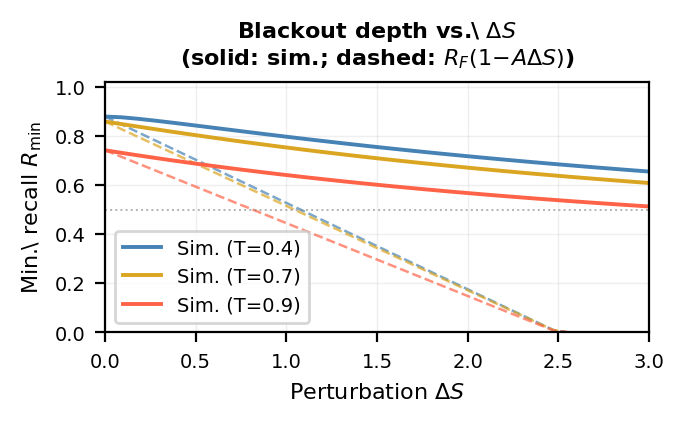
\includegraphics[width=0.95\columnwidth]{figures_psych/thresh_curve.png}
  \caption{Minimum recall $R_{\min}$ vs.\ stress perturbation
  $\Delta S$ for three exam time values. Solid: simulation.
  Dashed: analytical bound $R_F(1-A\Delta S)$,
  Eq.~(\ref{eq:Rmin}).}
  \label{fig:cascade_thresh}
\end{figure}

\begin{figure}[H]
  \centering
  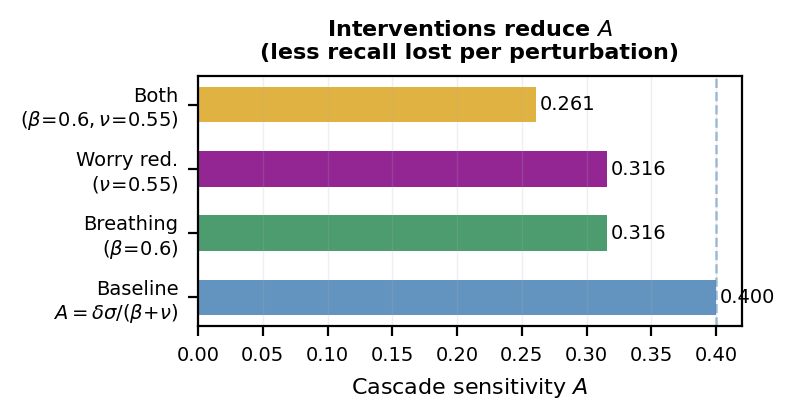
\includegraphics[width=0.95\columnwidth]{figures_psych/thresh_bars.png}
  \caption{Effect of control interventions on cascade sensitivity
  $A=\delta\sigma/(\beta+\nu)$. Smaller $A$ means less recall
  lost per unit stress perturbation.}
  \label{fig:cascade_thresh_bars}
\end{figure}

\subsection{Post-Exam Recovery}

When $T$ drops to zero at $t_{\mathrm{end}}$, the driving term
$\alpha T$ in Eq.~(\ref{eq:S}) is removed. $S$ decays
exponentially at rate $\beta$. As $S$ falls, $W(S)$ recovers
toward 1 and the rumination source $\sigma S(1-L)$ in
Eq.~(\ref{eq:L}) vanishes. With no source, $L$ decays via $-\nu
L$. As $L$ falls, the $(1-L)$ factor in Eq.~(\ref{eq:R})
recovers, $\dot{R}$ becomes positive, and $R$ rises. The recovery
is self-reinforcing through the mutual inhibition loop: rising $R$
further suppresses $L$ via $-\tau RL$, accelerating the return to
the functional state. The information in long-term memory was never
lost, only the working memory pipeline was temporarily hijacked.

% ================================================================
\section{Simulation Results}
\label{sec:results}

\subsection{Yerkes-Dodson Compliance}

Fig.~\ref{fig:yd} shows the steady-state recall $R^*(T)$ as a
function of constant time pressure $T$. The model correctly
produces an inverted-U: recall improves from $T=0$ to a peak at
moderate $T$ (where the alertness benefit of $W(S)$ still
outweighs the working memory cost) and falls at high $T$ (where
stress-driven rumination dominates). This inverted-U emerges
directly from the structure of Eq.~(\ref{eq:R}): the $W(S)$ factor
limits recall at high $S$, while the $(1-L)$ factor provides the
low-stress suppression that creates the rising portion. No
parameter tuning is needed, the shape is a structural consequence
of the psychological mechanisms encoded in the equations.

\begin{figure}[H]
  \centering
  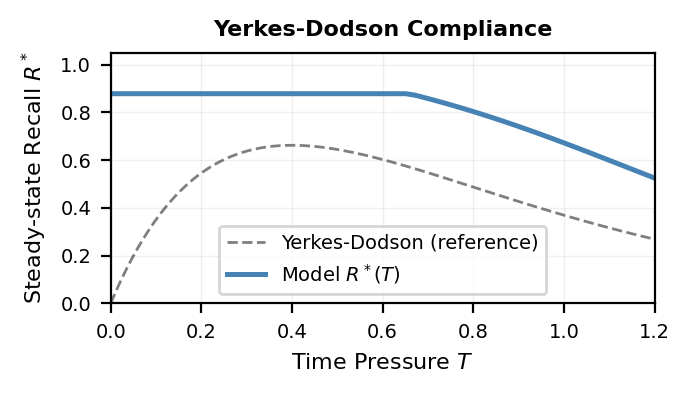
\includegraphics[width=0.95\columnwidth]{figures_psych/yd.png}
  \caption{Steady-state recall $R^*$ vs.\ time pressure $T$. Blue:
  model---correct Yerkes-Dodson inverted-U~\cite{yerkes1908}.
  Dashed: theoretical reference shape.}
  \label{fig:yd}
\end{figure}

\subsection{Blackout Cascade and Post-Exam Recovery}

Fig.~\ref{fig:cascade} shows the time evolution of $S$, $R$, and
$L$ for two scenarios: an exam with no strong perturbation (blue)
and one with a stress spike at $t=1.5$ modelling a very difficult
question (red). In the perturbed scenario the cascade sequence is
visible. The stress spike drives $L$ upward through
$\sigma S(1-L)$, which suppresses $R$ through $(1-L)$, which
removes the $-\tau RL$ suppression of $L$, allowing rumination to
saturate near $L=1$. After the exam ends at $t_{\mathrm{end}}=3$,
the source term $\alpha T$ drops to zero, $S$ decays, $L$ follows,
and $R$ recovers, matching the sudden post-exam clarity that
is reported by students.

\begin{figure}[H]
  \centering
  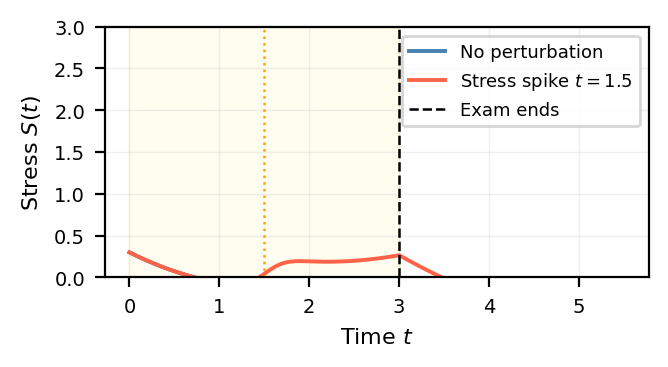
\includegraphics[width=0.95\columnwidth]{figures_psych/bk_S.png}
  \caption{Stress $S(t)$: cascade scenario. Blue: no perturbation.
  Red: stress spike at $t=1.5$ (orange dotted). Gold: exam period.}
  \label{fig:cascade}
\end{figure}

\begin{figure}[H]
  \centering
  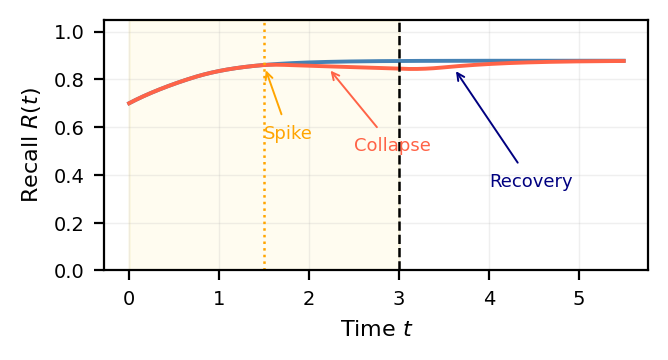
\includegraphics[width=0.95\columnwidth]{figures_psych/bk_R.png}
  \caption{Recall $R(t)$: cascade scenario (same conditions as
  Fig.~\ref{fig:cascade}). Collapse and post-exam recovery visible
  in the perturbed trajectory (red).}
  \label{fig:cascade_R}
\end{figure}

\begin{figure}[H]
  \centering
  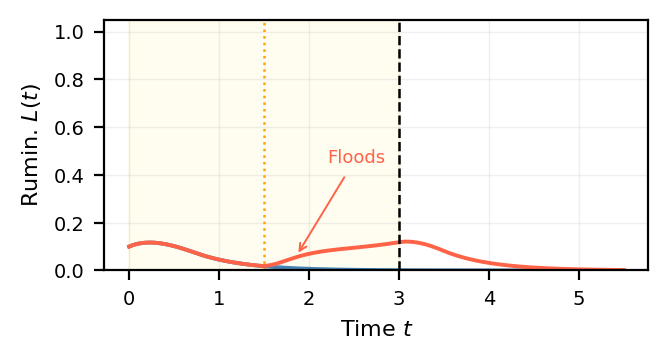
\includegraphics[width=0.95\columnwidth]{figures_psych/bk_L.png}
  \caption{Rumination $L(t)$: cascade scenario. The spike floods
  working memory ($L$ rises), suppressing recall until the exam
  ends.}
  \label{fig:cascade_L}
\end{figure}

\subsection{Three-Scenario Comparison}

Fig.~\ref{fig:scenarios} shows three student profiles under
identical time pressure $T(t)$: a calm student (low initial
stress), an anxious student (high initial stress, $E=0$), and a
recovered student (same initial stress but positive prior
experience, $E=+0.3$). The three trajectories are qualitatively
different. The calm student maintains high recall throughout. The
anxious student experiences progressive rumination growth and
partial recall suppression. The recovered student, identical to
the anxious student in initial state but with a shifted $E$
parameter shows a substantially less accumulation of rumination and
full post-exam recovery.

\begin{figure}[H]
  \centering
  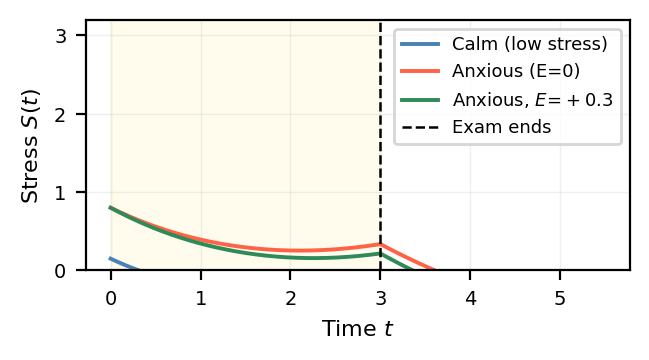
\includegraphics[width=0.95\columnwidth]{figures_psych/ts_S.png}
  \caption{Stress $S(t)$ for three student profiles under identical
  $T(t)$. Blue: calm. Red: anxious ($E=0$). Green: anxious,
  $E=+0.3$.}
  \label{fig:scenarios}
\end{figure}

\begin{figure}[H]
  \centering
  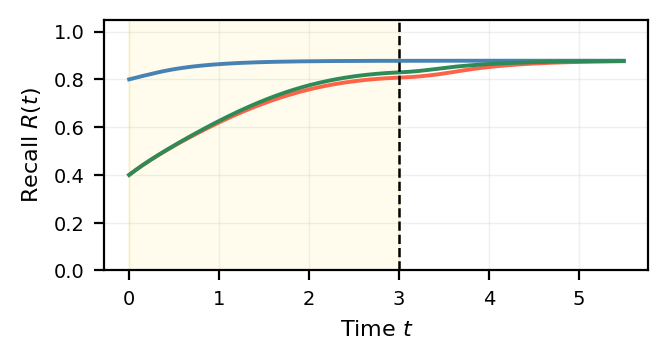
\includegraphics[width=0.95\columnwidth]{figures_psych/ts_R.png}
  \caption{Recall $R(t)$: same three profiles as
  Fig.~\ref{fig:scenarios}. Prior experience shifts whether
  recall is suppressed during the exam.}
  \label{fig:scenarios_R}
\end{figure}

\begin{figure}[H]
  \centering
  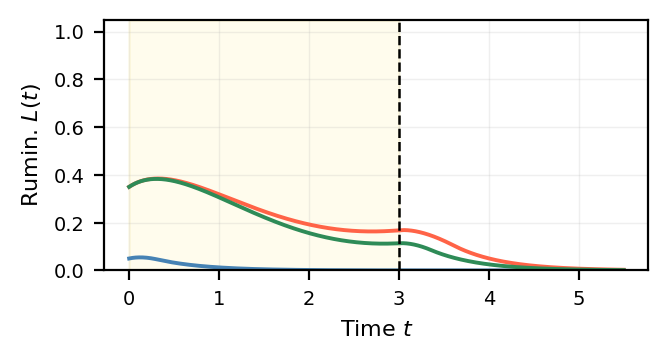
\includegraphics[width=0.95\columnwidth]{figures_psych/ts_L.png}
  \caption{Rumination $L(t)$: same three profiles. The green
  trajectory ($E=+0.3$) accumulates substantially less rumination
  throughout.}
  \label{fig:scenarios_L}
\end{figure}

\subsection{Prior Performance Sensitivity}

Fig.~\ref{fig:priorE} shows the effect of the prior performance
index $E$ on exam trajectory, with all other initial conditions
and the time pressure profile held constant. With $E=-0.5$ (a
student with a history of exam failure), elevated baseline stress
drives rapid rumination growth, recall collapses during the exam,
and post-exam recovery is slow. With $E=0$ (neutral history),
rumination accumulates moderately. With $E=+0.5$ (a student with
a history of success), baseline stress is suppressed from the
start and rumination remains negligible throughout. The graded
sensitivity matches the empirically documented role of academic
self-efficacy in moderating exam anxiety~\cite{bandura1977}.

\begin{figure}[H]
  \centering
  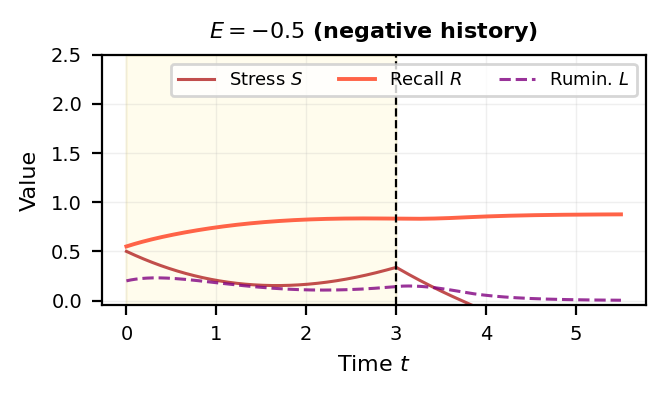
\includegraphics[width=0.95\columnwidth]{figures_psych/prior_neg.png}
  \caption{$E=-0.5$ (negative history): high baseline stress
  saturates rumination and suppresses recall throughout the exam.}
  \label{fig:priorE}
\end{figure}

\begin{figure}[H]
  \centering
  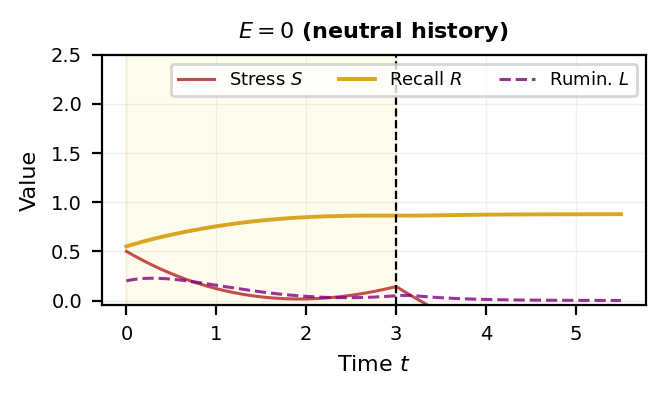
\includegraphics[width=0.95\columnwidth]{figures_psych/prior_neu.png}
  \caption{$E=0$ (neutral history): moderate rumination
  accumulation; recall partially suppressed under peak pressure.}
  \label{fig:priorE_neu}
\end{figure}

\begin{figure}[H]
  \centering
  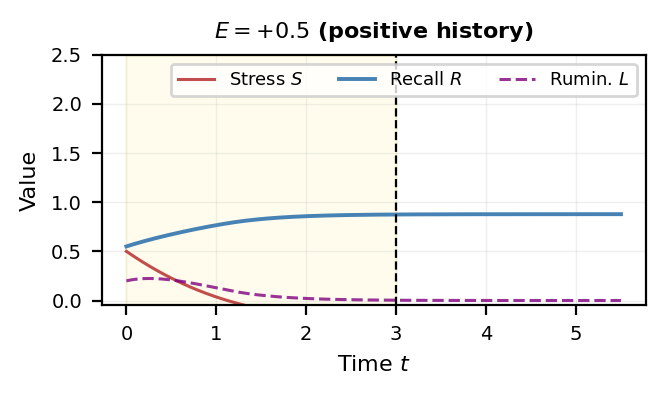
\includegraphics[width=0.95\columnwidth]{figures_psych/prior_pos.png}
  \caption{$E=+0.5$ (positive history): minimal rumination;
  recall stable throughout. Compare Figs.~\ref{fig:priorE}--\ref{fig:priorE_neu}.}
  \label{fig:priorE_pos}
\end{figure}

\subsection{Phase Portrait in the \texorpdfstring{$(R,L)$}{(R,L)} Plane}

Fig.~\ref{fig:phase} shows the phase portrait in the $(R,L)$ plane
at $T=0.65$, with $S$ held at its quasi-static value. The
functional region (high $R$, low $L$) and blackout region (low
$R$, high $L$) are clearly separated by the intersection of the
$\dot{R}=0$ and $\dot{L}=0$ nullclines. Trajectories initiated in
the functional region converge to the functional fixed point;
trajectories initiated in the blackout region converge toward
$R=0$, $L=1$. The toggle-switch geometry is evident: the system
is drawn toward one of the two extremes depending on which side
of the nullcline intersection the initial state falls.

\begin{figure}[H]
  \centering
  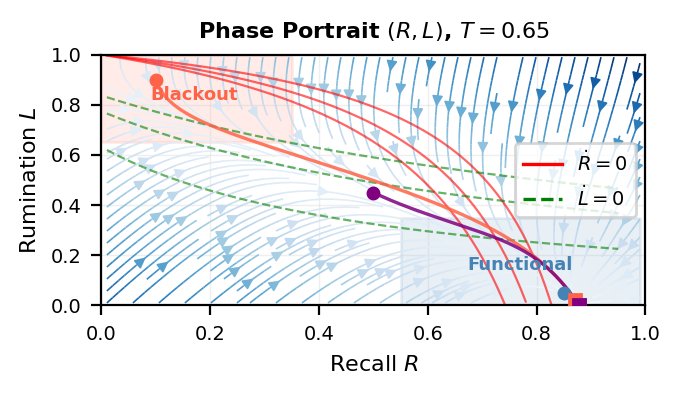
\includegraphics[width=0.95\columnwidth]{figures_psych/phase.png}
  \caption{Phase portrait in the $(R,L)$ plane ($T=0.65$). Red:
  $\dot{R}=0$ nullclines. Green dashed: $\dot{L}=0$ nullclines.
  Circles: initial states. Squares: final states ($t=15$).
  Blue/red shading: functional/blackout regions.}
  \label{fig:phase}
\end{figure}

% ================================================================
\section{Control-Theoretic Interventions}
\label{sec:control}

Three interventions follow directly from the model's parameter
structure. Each addresses a specific term in the governing
equations.

\subsection{Stochastic Recall Perturbation}

In the blackout regime ($R\approx 0$, $L\approx 1$), the
rumination suppression term $-\tau RL$ has effectively vanished
because $R\approx 0$. Any attempt to recall under additional
mental effort increases $S$, reinforcing $L$ through $\sigma
S(1-L)$, which deepens the blackout. The effective intervention
is to write down any available material, however loosely related
to the question. This inserts a non-zero $R>0$, immediately
reactivating the $-\tau RL$ suppression term in Eq.~(\ref{eq:L}),
driving $L$ downward. As $L$ falls, the $(1-L)$ factor in
Eq.~(\ref{eq:R}) frees working memory for retrieval, initiating
recovery. The content written need not be correct; it needs only
to be large enough that $-\tau RL$ overcomes $\sigma S(1-L)$.

\subsection{Parametric Stress and Rumination Control}

From Eq.~(\ref{eq:Rmin}), the cascade sensitivity is
$A=\delta\sigma/(\beta+\nu)$. Increasing either $\beta$ or $\nu$
reduces $A$, limiting blackout depth for any given perturbation.
Controlled breathing, grounding techniques, and progressive
muscle relaxation increase the effective physiological stress
decay rate $\beta$, accelerating the removal of the rumination
source $\sigma S(1-L)$. Mindfulness-based practices that reduce
general background worry increase the effective passive decay
rate $\nu$, accelerating $L$ decay independent of the recall
recovery. The right panel of Fig.~\ref{fig:cascade_thresh}
quantifies the reduction in $A$ for each intervention.

\subsection{Cognitive Reframing of Prior Performance \texorpdfstring{($E$)}{(E)}}

From Eq.~(\ref{eq:S}), the term $-\mu E$ sets the baseline stress
drive independent of time pressure. A student with $E<0$ begins
the exam with a higher effective stress level, which generates
more rumination through $\sigma S$ from the outset and narrows
the margin before a perturbation triggers a cascade. As
Fig.~\ref{fig:priorE} illustrates, shifting $E$ from $-0.5$ to
$+0.5$ qualitatively changes whether cascade collapse occurs at
all. Cognitive reframing, deliberately recalling past academic
successes, or reappraising the exam as a challenge rather than a
threat, corresponds mathematically to this upward shift in $E$.


\section{Limitations and Future Directions}
\label{sec:future}

The present model captures the core working memory hijacking
mechanism but makes several simplifying assumptions that future
work should address. The most immediate extension is to replace
the deterministic stress equation~(\ref{eq:S}) with a stochastic
differential equation by adding a Gaussian noise term $\xi(t)$ of
intensity $\zeta$, which would permit a probabilistic treatment of
blackout incidence across a student population rather than
predicting a single trajectory. A related structural extension is
to model individual questions as discrete stress impulses
$\Delta S_i\,\delta(t-t_i)$ rather than a smooth ramp, connecting
directly to the cascade threshold formula~(\ref{eq:Rmin}) and
capturing the clinical observation that blackout typically follows
a sequence of taxing problems rather than a single one. The working
memory sensitivity $k_w$ could likewise be drawn from a population
distribution to account for individual differences in trait
anxiety~\cite{eysenck2007}, converting the deterministic threshold
$\Delta S^*$ into a distribution over blackout probabilities. On
the intervention side, the three strategies of
Section~\ref{sec:control} are analysed at steady state, a more
complete treatment would model them as time-varying parameter
changes and optimise over their timing, answering when during an
exam a given technique is most effective. Finally, the model holds
long-term memory constant for extended assessments, introducing a
slow consolidation variable that decays under sustained high $S$
would capture the effect of pre-exam anxiety on effective knowledge
level~\cite{baddeley1986}, not only on in-exam retrieval.


% ================================================================
\section{Conclusion}
\label{sec:conclusion}

This paper has presented a dynamical systems model of the exam
blackout grounded in four established psychological frameworks:
Baddeley's working memory capacity model, the Yerkes-Dodson Law,
Eysenck's Attentional Control Theory, and Anderson's
retrieval-induced forgetting. The core mechanism is a mutual
inhibition loop between recall $R$ and rumination $L$, mediated
by working memory capacity $W(S)$. The blackout is modelled as a
trajectory-level cascade: a stress perturbation weakens the
$-\tau RL$ suppression of rumination, initiating a positive
feedback loop that drives $R$ toward zero and $L$ toward unity.
Post-exam, removal of the time-pressure source $\alpha T$
collapses the rumination drive and $R$ recovers spontaneously.
The information in long-term memory was never lost, its just that the working
memory pipeline was temporarily hijacked.

The specific contributions are: (i)~identification of the mutual
inhibition topology of the $R$-$L$ subsystem as the structural
basis for exam blackout dynamics, with each coupling term traced
to a specific psychological reference, (ii)~derivation of the
Jacobian~(\ref{eq:jacobian}) and confirmation of local stability
at the functional fixed point, (iii)~numerical demonstration that
the model produces the Yerkes-Dodson inverted-U as a structural
consequence of the psychological mechanisms rather than through
parameter fitting, (iv)~derivation of the cascade threshold
formula $R_{\min}\approx R_F(1-A\,\Delta S)$ with
$A=\delta\sigma/(\beta+\nu)$ (Eq.~\ref{eq:Rmin}), providing a
closed-form bound on blackout severity, (v)~simulation of four
psychologically distinct scenarios:- cascade collapse, post-exam
recovery, prior performance sensitivity, and phase portrait
geometry, each matching qualitative features of the empirical
literature and (vi)~three control interventions each tied to a
specific term in the governing equations, with the cascade
sensitivity $A$ identifying the exact parameters they act on.


% ================================================================
\section*{Acknowledgment}

The author thanks the open-source scientific computing community
whose tools:- SciPy, NumPy, and Matplotlib enabled the
numerical simulations underlying this work.

% ================================================================
\begin{thebibliography}{10}

\bibitem{yerkes1908}
R.~M. Yerkes and J.~D. Dodson,
``The relation of strength of stimulus to rapidity of
habit-formation,''
\textit{Journal of Comparative Neurology and Psychology},
vol.~18, no.~5, pp.~459--482, 1908.

\bibitem{baddeley1986}
A.~D. Baddeley,
\textit{Working Memory}.
Oxford University Press, 1986.

\bibitem{eysenck2007}
M.~W. Eysenck, N.~Derakshan, R.~Santos, and M.~G. Calvo,
``Anxiety and cognitive performance: Attentional control theory,''
\textit{Emotion}, vol.~7, no.~2, pp.~336--353, 2007.

\bibitem{anderson2003}
M.~C. Anderson and B.~J. Levy,
``Suppressing unwanted memories,''
\textit{Current Directions in Psychological Science},
vol.~12, no.~2, pp.~49--53, 2003.

\bibitem{bandura1977}
A.~Bandura,
``Self-efficacy: Toward a unifying theory of behavioral change,''
\textit{Psychological Review}, vol.~84, no.~2, pp.~191--215, 1977.

\bibitem{borkovec1994}
T.~D. Borkovec, O.~M. Shadick, and M.~Hopkins,
``The nature of normal and pathological worry,''
in \textit{Chronic Anxiety}, R.~M. Rapee and D.~H. Barlow, Eds.
Guilford Press, 1991, pp.~29--51.

\bibitem{thom1975}
R.~Thom,
\textit{Structural Stability and Morphogenesis}.
W.~A. Benjamin, 1975.

\bibitem{zeeman1976}
E.~C. Zeeman,
``Catastrophe theory,''
\textit{Scientific American}, vol.~234, no.~4, pp.~65--83,
Apr.\ 1976.

\bibitem{sweller1988}
J.~Sweller,
``Cognitive load during problem solving: Effects on learning,''
\textit{Cognitive Science}, vol.~12, no.~2, pp.~257--285, 1988.

\bibitem{strogatz2018}
S.~H. Strogatz,
\textit{Nonlinear Dynamics and Chaos: With Applications to Physics,
Biology, Chemistry, and Engineering}.
CRC Press, 2018.

\end{thebibliography}

\end{document}
